% !TeX program = xelatex 

\PassOptionsToPackage{prologue, dvipsnames}{xcolor}
\documentclass[AutoFakeBold,AutoFakeSlant]{article}
\usepackage{listings}

% 支持中文的设置
\usepackage{xeCJK}
\usepackage{fontspec}
\setCJKmainfont[ItalicFont=思源宋体,BoldFont=SourceHanSerifSC-Bold]{Source Han Serif SC}
\newcommand{\KaiTi}{\CJKfontspec{楷体}}%用命令\fzkaiti调用方正楷体简体

% other packages
\usepackage{subfigure}
\usepackage{latexsym,amsmath,xcolor,multicol,booktabs,calligra}
\usepackage{graphicx,pstricks,listings,stackengine}
\usepackage{quoting}
\usepackage{tcolorbox}

\usepackage{geometry}
\geometry{left=2cm,right=2cm,top=2cm,bottom=2cm}

\usepackage{hyperref}
\hypersetup
{
	colorlinks=true,
	linkcolor=blue,
	filecolor=blue,
	urlcolor=blue,
	citecolor=cyan,
}

\lstnewenvironment{x86asmcode}[1][]%
{
	\lstset{
		tabsize=4,
		breaklines=true,
		frame=shadowbox,
		breakatwhitespace=true, % 在空格处断行
		language={[x86masm]Assembler},
		escapeinside=``,
		basicstyle=\ttfamily,
		keywordstyle=\bfseries\color{NavyBlue},
		commentstyle=\itshape\color{black!50!white},
		literate={\ \ }{{\ \ \ \ }}4,
		#1
	}
}%
{}

\lstnewenvironment{cppcode}[1][]%
{
	\lstset{
		tabsize=4,
		language={C++},
		escapeinside=``,
		breaklines=true,
		frame=shadowbox, %把代码用带有阴影的框圈起来
		breakatwhitespace=true, % 在空格处断行
		basicstyle=\ttfamily,
		keywordstyle=\color{blue}\ttfamily,
		stringstyle=\color{red}\ttfamily,
		commentstyle=\color{green}\ttfamily,
		morecomment=[l][\color{magenta}]{\#},
		literate={\ \ }{{\ \ \ \ }}4,
		#1
	}
}%
{}

% 定义自定义命令来创建隐藏网址的超链接
\newcommand{\hiddenlink}[2]{%
	\href{#1}{\texttt{#2}}%
}

\begin{document}
	
	\vspace{3cm}
	\begin{center}
		\Huge 
		\textbf{ThinctDbg}用法说明书\\
		{\Large \textit{\underline{V1.0.0}}}
		
	\end{center}
	\vspace{1cm}
	
	\leftline
	\bigskip
	\begin{flushleft}
		\begin{Large}
			Windows 环境条件
		\end{Large}
		\large 
		\linespread{1.2} \selectfont
		\begin{quote}
			1. python3\\
			2. \hiddenlink {https://github.com/lyshark/LyScript} {LyScript32环境安装}.
			\begin{quote}安装之后,需要将其中的\hiddenlink{https://github.com/thinct/ThinctDbg/blob/main/\_\_init\_\_.py}{\_\_init\_\_.py}文件进行更新,主要是为了提升执行速度。
			\end{quote}
		\end{quote}
		
		\vspace{1cm}
		
		\begin{LARGE}
			一、 \textbf{RuntimeTrace} 运行时反汇编代码跟踪
		\end{LARGE}
		
		\large 
		\linespread{1.6} \selectfont
		\begin{quote}
			1. 脚本可以将运行过程中\textbf{执行过的反汇编代码}作为路径,按照要求记录下来。\\
			\begin{quotation}
				a. 直接阅读分析这样的单一路径的代码简单于庞杂的整体分析;\\
				b. 基于不同的输入,可以得到不同的执行路径;\\
				c. 可以综合多个路径来分析或猜测功能函数;\\
				d. IDA静态分析功能强大,借助路径分析可以更加方便分析反汇编代码。
			\end{quotation}
			\begin{quotation}
			记录会写入到AddrFlowEasy.asm文件中。在执行过程中,同样会\textbf{记录遇到的内存访问}。
			\end{quotation}
		
			\newpage
			
			\large 
			2. 脚本参数用法 \\
			\begin{quote}
				\textcolor{blue}{ \textbf{ \Large
				.$\backslash$RuntimeTrace.py $--$S 0x00402029 $--$E 0x0040206A $--$StepIn 0x00402064 $--$StepIn 0x68B09B26 --MustAddr 0x68B09B0A $--$PauseOnce 0x68B09B0A }}\\
				\begin{quote}
					%\begin{tcolorbox}
					\textbf{$--$S}
					\begin{quote} 指定分析的起点,\textbf{$--$E}指定分析的终点.也就是单步过程中必须要经过这两处地址.
					\end{quote}
					\textbf{$--$StepIn} 
					\begin{quote}
						指定的地址如果是遇到call的目标地址,就执行step in.
					\end{quote}
					\textbf{$--$MustAddr}
					\begin{quote}
					 指定的地址则必须执行到的地址,也就是说即使程序执行到$--$E指定的点,如果仍有MustAddr指定的地址没有达到,那么就继续执行.
					\end{quote}
					%\end{tcolorbox}
				\end{quote}
			
			\bigskip
			\bigskip
			
			\textcolor{blue}{ \textbf{ \Large
		    .$\backslash$RuntimeTrace.py $--$S 0x01071AD0 $--$E 0x01071BC1 $--$StartInModules 0x01060000 $--$EndInModules 0x01076FF2 }} \\
		    \begin{quote}
		    	%\begin{tcolorbox}
			    $--$S \begin{quote}指定分析的起点,$--$E指定分析的终点.也就是单步过程中必须要经过这两处地址.\end{quote}
			    $--$StepIn \begin{quote}指定的地址如果是遇到call的目标地址,那么就会执行step in.\end{quote}
			    \textbf{$--$StartInModules} \begin{quote}指定允许记录的模块起始点,\textbf{$--$EndInModules}指定允许记录的模块终点。如果step in和step out的地址在指定的模块范围内,就继续执行。否则会执行step out直到单步到允许的地址范围内。\end{quote}
			    %\end{tcolorbox}
			\end{quote}
		    
			\clearpage
		    
		    \textcolor{blue}{ \textbf{ \Large
			.$\backslash$RuntimeTrace.py $--$S 0x004011A0 $--$E 0x004012ED $--$StartInModules 0x00400000 $--$EndInModules 0x00402FFF $--$noEnablePrtESP }} \\
			\begin{quote}
				%\begin{tcolorbox}
				$--$S \begin{quote}指定分析的起点,$--$E指定分析的终点.也就是单步过程中必须要经过这两处地址.\end{quote}
				$--$StepIn \begin{quote}指定的地址如果是遇到call的目标地址,那么就会执行step in.\end{quote}
				$--$StartInModules \begin{quote}指定允许记录的模块起始点,$--$EndInModules指定允许记录的模块终点。如果step in和step out的地址在指定的模块范围内,就继续执行。否则会执行step out直到单步到允许的地址范围内。\end{quote}
				\textbf{$--$noEnablePrtESP} \begin{quote}执行反汇编的过程中,不记录ESP的值。\end{quote}
				%\end{tcolorbox}
			\end{quote}
			
			\bigskip			
			
			\textcolor{blue}{ \textbf{ \Large
			.$\backslash$RuntimeTrace.py $--$S 0x004011A0 $--$E 0x004012ED $--$StartInModules 0x00400000 $--$EndInModules 0x00402FFF $--$noEnablePrtESP --ModifyCallAddr }} \\
			\begin{quote}
				%\begin{tcolorbox}
				$--$S \begin{quote}指定分析的起点,$--$E指定分析的终点.也就是单步过程中必须要经过这两处地址.\end{quote}
				$--$StepIn \begin{quote}指定的地址如果是遇到call的目标地址,那么就会执行step in.\end{quote}
				$--$StartInModules \begin{quote}指定允许记录的模块起始点,$--$EndInModules指定允许记录的模块终点。如果step in和step out的地址在指定的模块范围内,就继续执行。否则会执行step out直到单步到允许的地址范围内。\end{quote}
				$--$noEnablePrtESP \begin{quote}执行反汇编的过程中,不记录ESP的值。\end{quote}
				\textbf{--ModifyCallAddr} \begin{quote}将call的目标地址修改。比如call 0x12345678改成mov eax,0x12345678和call eax. \end{quote}
			    %\end{tcolorbox}
			\end{quote}
			
			\end{quote}
		
			\newpage	
		
			\begin{quote}
				3. 下面展示的是记录文件AddrFlowEasy.asm的部分内容:
				\begin{quote}
				\begin{x86asmcode}
;esp : 0x0019FD1C
;ebp : 0x0019FE0C
/*0x00411959*/    rep stosd
/*0x0041195B*/    mov ecx, 0x41C00D
/*0x00411960*/    call 0x0041132F
;esp : 0x0019FD18
;/*0x0041132F*/    jmp 0x004119D0
/*0x004119D0*/    push ebp
;esp : 0x0019FD14
/*0x004119D1*/    mov ebp, esp
;ebp : 0x0019FD14
/*0x004119D3*/    sub esp, 0x8
;esp : 0x0019FD0C
/*0x004119D6*/    mov dword ptr ss:[ebp-0x4], ecx
;[ebp-0x4]=[0x0019FD10]=0x0019FD18
;[ebp-0x4]=[0x0019FD10]=0x0041C00D  <-- Modify
/*0x004119D9*/    mov eax, dword ptr ss:[ebp-0x4]
;[ebp-0x4]=[0x0019FD10]=0x0041C00D
/*0x004119DC*/    mov dword ptr ss:[ebp-0x8], eax
;[ebp-0x8]=[0x0019FD0C]=0x00288000
;[ebp-0x8]=[0x0019FD0C]=0x0041C00D  <-- Modify
/*0x004119DF*/    mov ecx, dword ptr ss:[ebp-0x4]
;[ebp-0x4]=[0x0019FD10]=0x0041C00D
/*0x004119E2*/    movzx edx, byte ptr ds:[ecx]
;[ecx]=[0x0041C00D]=0x00000101
				\end{x86asmcode}
				\end{quote}
			\end{quote}
		\end{quote}
	\end{flushleft}
	
	\newpage
	
	\begin{flushleft}
		\begin{LARGE}
			二、 \textbf{IDAAnalyze} 获取IDA中的反汇编代码
		\end{LARGE}
		
		\bigskip
		\bigskip
		
		\large 
		\linespread{1.6} \selectfont
		\begin{quote}
		遍历IDA所加载模块的所有函数的反汇编代码。按照如下格式保存到了C:$\backslash$$\backslash$DisasmSet文件中:
		\begin{x86asmcode}
	0x004125FD    jz      short loc_41260D
	0x004125FF    call    ds:IsDebuggerPresent
	0x00412605    test    eax, eax
	0x00412607    jnz     loc_41270C
	0x0041260D    push    104h; unsigned int
	0x00412612    lea     eax, [ebp+var_414]
	0x00412618    push    eax; wchar_t *
	0x00412619    lea     eax, [ebp+var_E38]
	0x0041261F    push    eax; int *
	0x00412620    push    104h; char
	0x00412625    lea     eax, [ebp+var_20C]
	0x0041262B    push    eax; wchar_t *
	0x0041262C    lea     eax, [esi-5]
	0x0041262F    push    eax; unsigned __int8 *
		\end{x86asmcode}
		
		目前这样的输出文件,被后面章节的BreakpointTool使用。因为使用X64 Dbg的LyScript来分析机器码对应的反汇编时,经常会出现错误,分析出的反汇编代码,在x64dbg实际的代码段中并没有出现。那么可以借助这里得到的反汇编代码进行比对来进行纠错。
		\end{quote}
	\end{flushleft}
	
	\newpage
	
	\begin{flushleft}
		\begin{LARGE}
			三、 \textbf{BreakpointTool} 设置断点探查消息处理函数
		\end{LARGE}
		
		\large 
		\linespread{1.6} \selectfont
		
		\begin{quote}
			\textcolor{blue}{ \textbf{ \Large
					.$\backslash$python BreakpointTool.py $--$S 0x400000 $--$E 0x410000 \\$--$Step 100 }}
			\begin{quote}
				%\begin{tcolorbox}
				\textbf{$--$S}
				\begin{quote} 指定分析的起点,\textbf{$--$E}指定分析的终点.也就是单步过程中必须要经过这两处地址.
				\end{quote}
				\textbf{$--$E} 
				\begin{quote}
					指定的地址如果是遇到call的目标地址,就执行step in.
				\end{quote}
				\textbf{$--$Step}
				\begin{quote}
					指定的地址则必须执行到的地址,也就是说即使程序执行到$--$E指定的点,如果仍有MustAddr指定的地址没有达到,那么就继续执行.
				\end{quote}
				%\end{tcolorbox}
			\end{quote}
			
			\bigskip
			
			按照指定的范围,提取地址和对应的反汇编代码。不过在这个提取过程是需要将DisasmSet文件中的代码与X64 Dbg提取的反汇编代码进行比对,只有两者在地址一致且对应的反汇编代码的操作码一致的情况下才作为设置断点的有效代码。
			
		\end{quote}
		
	\end{flushleft}
	
	\newpage
	
	\begin{flushleft}
		\begin{LARGE}
			四、 \textbf{RuntimeTrace IDAAnalyze BreakpointTool}结合使用 
		\end{LARGE}
		\large 
		\linespread{1.6} \selectfont
		
		\begin{enumerate}
			\item 修改PE的DllCharacteristics禁用ASLR
				{
					\small
					\begin{quote}
						使用\hiddenlink {https://bbs.kanxue.com/thread-279901.htm} {修改PE的DllCharacteristics禁用ASLR }.提到的代码来进行修改固定基址.
					\end{quote}
				}
			\item 使用IDAAnalyze导出分析文件的反汇编代码信息(地址+反汇编指令)
				{
					\small
					\begin{quote}
						使用脚本执行之后,会导出反汇编格式的信息到 \textit{C:/DisasmSet} 文件中。大致是这样子的:
\begin{x86asmcode}
0x00401000    push    ebp
0x00401001    mov     ebp, esp
0x00401003    push    esi
0x00401004    mov     esi, ecx
0x00401006    xorps   xmm0, xmm0
0x00401009    lea     eax, [esi+4]
0x0040100C    push    eax
0x0040100D    mov     dword ptr [esi], offset ??_7exception@std@@6B@
0x00401013    movq    qword ptr [eax], xmm0
0x00401017    mov     eax, [ebp+arg_0]
0x0040101A    add     eax, 4
0x0040101D    push    eax
0x0040101E    call    ds:__std_exception_copy
0x00401024    add     esp, 8
0x00401027    mov     eax, esi
0x00401029    pop     esi
0x0040102A    pop     ebp
0x0040102B    retn    4
;-------------------------------------------
0x00401030    lea     eax, [ecx+4]
0x00401033    mov     dword ptr [ecx], offset ??_7exception@std@@6B@
0x00401039    push    eax
0x0040103A    call    ds:__std_exception_destroy
0x00401040    pop     ecx
0x00401041    retn
;-------------------------------------------\end{x86asmcode}
					\end{quote}
				}
			\item 使用BreakpointTool设置要分析代码的大致范围的断点
			
			\newpage
			
			\item 使用X64Dbg动态调试,只保留关注函数的入口断点。删除其他断点,禁用频繁触发的断点
				{
					\small
					\begin{enumerate}
						\item 耐心的F9运行代码
						\item 在没有运行到自己感兴趣的功能时,可以清除已经被击中的断点,一般这种断点很大可能时和感兴趣代码是无关的代码片段
						\item 在运行到自己感兴趣的功能时,关注被击中的断点,这种断点一般就是自己要分析的反汇编对象,但是有些明显被频繁触发的反汇编区域,可以暂时屏蔽该断点。一般这种断点可能是某种刷新函数,所以为了不妨碍接下来的F9分析其他相关函数击中断点的进度,就暂时屏蔽跳过。
						\item 在自己感兴趣的功能运行结束或者快要结束时,可以将未被击中的断点全部删除掉,因为这块逻辑很大概率时和当前要分析的对象时无关的。
						\begin{flushleft}
							\begin{figure*}[htbp]
								\centering
								\subfigure[找到了感兴趣功能被命中的断点]{
									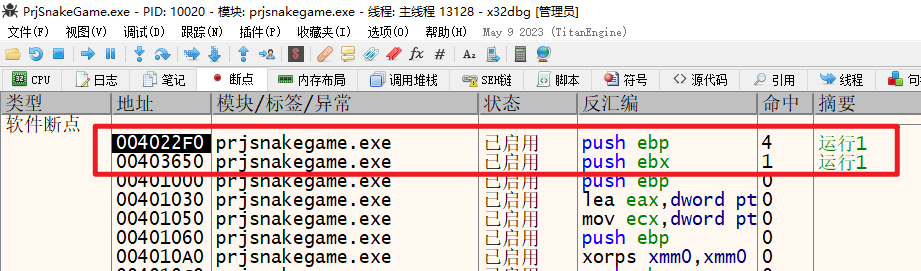
\includegraphics[width=0.8\linewidth]{X64DbgBpsFilter01}
								} 
							\end{figure*}
							在后面一次都没有命中的断点,可以考虑将这些断点全部删除掉。使分析问题的思路更加聚焦。退一步讲,如果担心有些断点删除会疏忽掉,可以在删除之前将环境保存到数据库.
						\end{flushleft}
					\end{enumerate}
					通过上面的流程仔细筛选,基本能找到要分析功能相关的几个要分析的函数了。接下来就要分化任务了:
					\begin{enumerate}
						\item 将筛选过的断点保存数据库
						\item 留下一个函数入口附近的有效断点。保证运行的时候会被击中。
						\item 观察分析函数的最大范围。
					\end{enumerate}
				}
			\item 使用RuntimeTrace自动step over关注的函数区域,其他区域进行step run.
				{
					\small
					\begin{enumerate}
						\item 根据上面分析出来的函数最大范围进行运行
						\item 观察导出的 \textit{AddrFlowEasy.asm} 文件,分析程序流程和数据变化,进行逆向分析
						\item 结合IDA的反汇编代码对比分析
					\end{enumerate}
				}
			\item 实战命令顺序.
				{
					
					\small
					BreakpointTool.py
					\begin{enumerate}
						\item python .$\backslash$BreakpointTool.py $--$S 0x400000 $--$E 0x410000 $--$Step 10
						\item echo Running>ExternMsg.txt
						\item yes
						\item echo Reset>ExternMsg.txt
						\item echo Over>ExternMsg.txt
					\end{enumerate}
					RuntimeTrace.py
					删除一些没有命中过的断点
					\begin{enumerate}
						\item python.exe .$\backslash$RuntimeTrace.py $--$S 0x00403650 $--$E 0x00403B37 $--$EnableFastMode $--$EnableSnapMode
						\item echo SnapStart>ExternMsg.txt
						\item echo Over>ExternMsg.txt
					\end{enumerate}
					要注意的是,尽量在靠近功能断点附近开启SnapStart模式,在功能结束之后输入Over.
				}
		\end{enumerate}
	\end{flushleft}
		
\end{document}
